% This is "sig-alternate.tex" V2.1 April 2013
% This file should be compiled with V2.5 of "sig-alternate.cls" May 2012
%
% This example file demonstrates the use of the 'sig-alternate.cls'
% V2.5 LaTeX2e document class file. It is for those submitting
% articles to ACM Conference Proceedings WHO DO NOT WISH TO
% STRICTLY ADHERE TO THE SIGS (PUBS-BOARD-ENDORSED) STYLE.
% The 'sig-alternate.cls' file will produce a similar-looking,
% albeit, 'tighter' paper resulting in, invariably, fewer pages.
%
% ----------------------------------------------------------------------------------------------------------------
% This .tex file (and associated .cls V2.5) produces:
%       1) The Permission Statement
%       2) The Conference (location) Info information
%       3) The Copyright Line with ACM data
%       4) NO page numbers
%
% as against the acm_proc_article-sp.cls file which
% DOES NOT produce 1) thru' 3) above.
%
% Using 'sig-alternate.cls' you have control, however, from within
% the source .tex file, over both the CopyrightYear
% (defaulted to 200X) and the ACM Copyright Data
% (defaulted to X-XXXXX-XX-X/XX/XX).
% e.g.
% \CopyrightYear{2007} will cause 2007 to appear in the copyright line.
% \crdata{0-12345-67-8/90/12} will cause 0-12345-67-8/90/12 to appear in the copyright line.
%
% ---------------------------------------------------------------------------------------------------------------
% This .tex source is an example which *does* use
% the .bib file (from which the .bbl file % is produced).
% REMEMBER HOWEVER: After having produced the .bbl file,
% and prior to final submission, you *NEED* to 'insert'
% your .bbl file into your source .tex file so as to provide
% ONE 'self-contained' source file.
%
% ================= IF YOU HAVE QUESTIONS =======================
% Questions regarding the SIGS styles, SIGS policies and
% procedures, Conferences etc. should be sent to
% Adrienne Griscti (griscti@acm.org)
%
% Technical questions _only_ to
% Gerald Murray (murray@hq.acm.org)
% ===============================================================
%
% For tracking purposes - this is V2.0 - May 2012

\documentclass{report}

\usepackage{url}

\begin{document}

% Copyright
%\setcopyright{acmcopyright}
%\setcopyright{acmlicensed}
%\setcopyright{rightsretained}
%\setcopyright{usgov}
%\setcopyright{usgovmixed}
%\setcopyright{cagov}
%\setcopyright{cagovmixed}


% DOI
%\doi{10.475/123_4}

% ISBN
%\isbn{123-4567-24-567/08/06}

%Conference
%\conferenceinfo{PLDI '13}{June 16--19, 2013, Seattle, WA, USA}

%\acmPrice{\$15.00}

%
% --- Author Metadata here ---
%\conferenceinfo{WOODSTOCK}{'97 El Paso, Texas USA}
%\CopyrightYear{2007} % Allows default copyright year (20XX) to be over-ridden - IF NEED BE.
%\crdata{0-12345-67-8/90/01}  % Allows default copyright data (0-89791-88-6/97/05) to be over-ridden - IF NEED BE.
% --- End of Author Metadata ---

\title{Mining Requirements Traces : A Decade Long Journey}
%
% You need the command \numberofauthors to handle the 'placement
% and alignment' of the authors beneath the title.
%
% For aesthetic reasons, we recommend 'three authors at a time'
% i.e. three 'name/affiliation blocks' be placed beneath the title.
%
% NOTE: You are NOT restricted in how many 'rows' of
% "name/affiliations" may appear. We just ask that you restrict
% the number of 'columns' to three.
%
% Because of the available 'opening page real-estate'
% we ask you to refrain from putting more than six authors
% (two rows with three columns) beneath the article title.
% More than six makes the first-page appear very cluttered indeed.
%
% Use the \alignauthor commands to handle the names
% and affiliations for an 'aesthetic maximum' of six authors.
% Add names, affiliations, addresses for
% the seventh etc. author(s) as the argument for the
% \additionalauthors command.
% These 'additional authors' will be output/set for you
% without further effort on your part as the last section in
% the body of your article BEFORE References or any Appendices.

\numberofauthors{1} %  in this sample file, there are a *total*
% of EIGHT authors. SIX appear on the 'first-page' (for formatting
% reasons) and the remaining two appear in the \additionalauthors section.
%
\author{
% You can go ahead and credit any number of authors here,
% e.g. one 'row of three' or two rows (consisting of one row of three
% and a second row of one, two or three).
%
% The command \alignauthor (no curly braces needed) should
% precede each author name, affiliation/snail-mail address and
% e-mail address. Additionally, tag each line of
% affiliation/address with \affaddr, and tag the
% e-mail address with \email.
%
% 1st. author
\alignauthor
    George Mathew\\
    \affaddr{Department of Computer Science}\\
    \affaddr{North Carolina State University}\\
    \affaddr{Raliegh, NC, USA}\\
    \email{george2@ncsu.edu}
}
% There's nothing stopping you putting the seventh, eighth, etc.
% author on the opening page (as the 'third row') but we ask,
% for aesthetic reasons that you place these 'additional authors'
% in the \additional authors block, viz.
% Just remember to make sure that the TOTAL number of authors
% is the number that will appear on the first page PLUS the
% number that will appear in the \additionalauthors section.

\maketitle
\begin{abstract}
Requirements traceability is a critical software engineering activity that 
provides support for numerous tasks such as impact analysis, compliance verification
and coverage analysis. Automated trace retrieval methods came into prominence since 
early 2000s and significantly reduced the
cost and effort needed to create and maintain requirements traces. 
These techniques generates low precision and is augmented with manual evaluation with business analysts.
In this report, a study is performed to review various techniques used in the last decade to mine
traces. These techniques are mostly automated with some of them using manual augmentation to filter
the queries. The report also describes the datasets used to evaluate these
techniques and suggests what the road ahead in requirements traceability looks like for
the next decade.
\end{abstract}

% We no longer use \terms command
%\terms{Theory}

\keywords{\textbf{Requirements, Information Retrieval, Requirements Traceability, Text Mining, Machine Learning}}

\section{Introduction}
Requirements traceability is defined as the ability to track the life of a requirement
back to its source documents and forward to the downstream work
products in which it is realized \cite{hayes94}. Traceability links are
generally created and maintained by project stakeholders using
spreadsheets, databases, or specialized trace features of
commercial requirements management tools. However, in nontrivial
projects, the number of traceability links can grow very large, 
and as a result the manual effort required to establish and
maintain such traces is often inhibitive.

Various different approaches were used for information retrieval in dynamically
generating traceability links. Most of the popular approaches have utilized 
Vector Space Modelling (VSM) \cite{hayesVSM06}, probabilistic approaches \cite{clelandHuang05} or 
Latent Semantic Indexing(LSI) \cite{antoniol02, LSI00}. Prior to these techniques, standard software
engineering practices of requirements traceability were used which refers to ``the ability to track 
a requirement from its origins back to its rationale and downstream to various work products
that implement the requirement is software"\cite{gotel94}. To trace the requirements, software
developers are often forced to manually pore over documentation manuals to identify relevant sections 
and then painstakingly trace them to product level requirements or implemented code. These traces
are typically represented in trace matrices.

In this paper, we discuss various techniques for automatically obtaining requirement traces. Section \ref{sec:relatedWork} highlights the work prior to the year 2002. Section \ref{sec:codeAndDoc} starts of with retrieving traceability links between code and documentation. 
Section \ref{sec:dynamicReq} discusses utilizing support evidence for improving dynamic requirements traceability.
Sections \ref{sec:wikipedia}, \ref{sec:MLTechs} and \ref{sec:SEAugment} discusses utilizing wikipedia, machine
learning techniques and search engines to improve user's query intents. Further, sections \ref{sec:enhanceCandidates},
\ref{sec:queryReformulate} and \ref{sec:intelligentTraces}
highlights enhancement of candidate links, reformulating queries to yield better results and techniques for more
intelligent trace retrievals. We finally conclude highlighting the datasets used in the studies in Section \ref{sec:datasets} followed by scope for future work in this domain in Section \ref{sec:future}.

\section{Related Work}
\label{sec:relatedWork}
In early to mid 2000s, trace retrieval started moving towards dynamic approaches from manual ones\cite{antoniol02, hayes03, hayes94, settimi04}. These approaches were based on information retrieval methods that link artifacts based on the occurrence of terms in both the requirement and set of traceable documents on the structure of terms used in the grammar. These methods usually predict high recall levels (close to 90\%) but the precision rates were vary low typically in the range of 10\% to 45\%.

Another school of thought is the assumption of existence of some form of ripple propagation graph describing relations between software artifacts, including code and documentation, and focus on the prediction of the effects of maintenance change request on both the source code and design documents \cite{arnold93, fyson98}. Prior attempts to retrieve source code and design documents that involve a hybrid approach that integrates logic based static and dynamic visualization and helps determining design-implementation congruence at various levels of abstraction was proposed by \textit{Sefika et al.} \cite{sefika96}

Analysis of informal information in the source code (comments and mnemonics for identifiers) can help to associate domain concepts with program fragments and vice-versa. The importance of informal information analysis has been discussed in \cite{biggerstaff89} where an approach based on structures similar to semantic networks was proposed and the possibility of using some kind of neural networks had been suggested. Comments and mnemonics are known to have an information content with an extremely large degree of variance between systems and, often, between different segments of the same system.

\section{Requirements Traceability}
\subsection{Code \& Documentation Traceability}
\label{sec:codeAndDoc}

Code and Document traceability was explored by \textit{Antoniol et al.} \cite{antoniol02} in their 2002
publication in IEEE Transactions of Software Engineering.

\begin{figure*}[!ht]
\begin{minipage}{\linewidth}
\centering
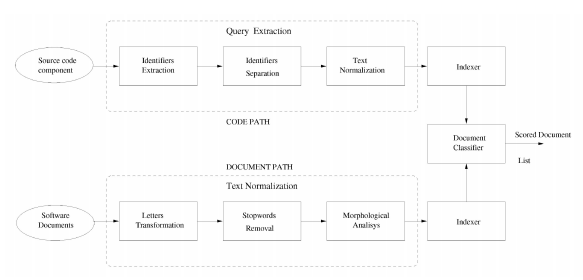
\includegraphics[scale=0.75]{img/traceability-links}
\caption{Traceability Link Recovery Method.}
\label{fig:traceLinks}
\end{minipage}
\end{figure*}

Traceability links play a vital role in acquiring data for requirements. Links
between areas of code and related sections of free text documents, such as an
application domain handbook, a specification document, a set of design documents, or manual pages, 
aid both top-down and bottom-up comprehension. The links between code and other sources of
information are a sensible help to perform the combined analysis of heterogeneous information and,
ultimately, to associate domain concepts with code fragments. Traceability links between the
requirement specification document and the code are a key to locate the areas of code that contribute
to implement specific user functionality. This helps assess the completeness of an implementation with
respect to stated requirements, to devise complete and comprehensive test cases, and to infer
requirement coverage from structure coverage during testing. Traceability links between requirements
and code can also help to identify the code areas directly affected by a maintenance request as stated
by an end user. Tracing code to free text documents are a sensible help to locate reused candidate
components. Traceability Links are retrieved as shown in Figure \ref{fig:traceLinks}.

In their work, recovering traceability links between free text documentation and
source-code components cannot be simply based on compiler techniques because of the
difficulty of applying syntactic analysis to natural language sentences. Hence the
premise of their work is that programmers use meaningful names for program items,
such as functions, variables, types, classes, and methods. The analysis of mnemonics
can help to associate high-level concepts with program concepts, and vice-versa. The
names of program items are used as a clue to suggest concepts implemented in the
code. After this preprocessing they, propose two different methods, a
Probabilistic IR Model \& Vector Space IR Model.

\textbf{Probabilistic Information Retrieval Model : } In this model free-text
documents are ranked according to the probability of being relevant to a query
computed on a statistical basis. To compute this ranking, the idea of a language
model is exploited, i.e., a stochastic model that assigns a probability to every
string of words taken from a prescribed vocabulary. A language model is estimated for
each document, or identifiable section, and use a Bayesian classifier to score the
sequences of mnemonics extracted from each source code component against the models.
A high score indicates a high probability that a particular sequence of mnemonics be
relevant to the document; therefore, it is interpreted as an indication of the
existence of a semantic link between the component from which the sequence had been
extracted and the document.

\textbf{Vector Space Information Retrieval Model : } Vector space IR models map each
document and each query onto a vector \cite{rankingAlgosHarman92}. Vector space model
treats documents and queries as vectors in an n-dimensional space, where n is the
number of indexing features. Documents are ranked against queries by computing a
distance function between the corresponding vectors. In their work, the documents are
ranked according to a widely used distance function, i.e., the cosine of the angle
between the vectors. For information retrieval the metric \textit{tf-idf} \cite{saltonTFIDF88} is used where the ${j}^{th}$ element $d_{i,j}$ is
derived from the term frequency $tf_{i,j}$ of the $j^{th}$ term in the document
$D_{i}$ and the inverse document frequency $idf_j$ of the term over
the entire set of documents. The term frequency $tf_{i,j}$ is the
ratio between the number of occurrences of word $j^{th}$ over
the total number of words contained in the document $D_i$.
The inverse document frequency $idf_j$ is defined as:

\[ idf_j = \frac{\textit{Total Number of Documents}}{\textit{Number of Documents containing the $j^{th}$ term.}} \]

This paper was one the first approaches taken by the research community to move 
towards automatically fetch requirement traces. This explains why the authors have
taken to such basic model generation like Probabilistic IR model and Vector Space IR
model. But the paper fails to address the intuition behind how the probabilistic model is constructed. Barring this drawback, the paper sets a strong benchmark for
the community and is well justified as one of the most cited papers in the domain
of requirements engineering. 


\subsection{Dynamic Requirements Traceability}
\label{sec:dynamicReq}
Requirements traceability provides critical support
throughout all phases of a software development project.
However, practice has repeatedly shown the difficulties
involved in long-term maintenance of traditional
traceability matrices. This was the premise of the work of 
\textit{Cleland-Huang et al.} in their 
2005 publication in IEEE International Conference on Requirements
Engineering\cite{clelandHuang05}. 

Dynamic retrieval methods minimize the need for creating and maintaining explicit links and can
significantly reduce the effort required to perform a manual trace. These methods have recall and
precision problems. Typical industrial practices in which traceability matrices are manually
constructed and maintained tend to be costly to implement and are financially non-viable. Current
research has investigated the use of dynamic retrieval methods to automate the process of generating
traceability links. These approaches are based on information retrieval methods that link artifacts
according to the occurrence of terms in both the requirement and set of searchable documents or on the
grammatical structuring of the terms. Results from these approaches are promising because they clearly
demonstrate the feasibility of replacing traditional trace methods with dynamic ones, but
unfortunately they also suffer from precision problems. 

The method proposed by the authors uses manually created traceability matrices to train a trace
classifier, while another method uses web mining techniques to reconstruct the original trace
query.Machine learning methods are particularly appealing for tracing regulatory codes, because the
upfront effort of training a classifier can be potentially recouped when those same codes are applied
across future projects. When a training set is not available, web mining approach can be used to
retrieve relevant set of indicator terms from the internet. This method augments the predictions by
machine learning approach. In hierarchical enhancement ancestors that are closer to the query q are
likely to provide stronger information about the query, compared to other ancestors that lay farther
away in the query hierarchy. Clustering enhancements are based on the premise that links tend to occur
in clusters. If a link exists between a query and a document, and if that document is part of a
logical cluster of documents, then there would be a higher probability that additional links should
exist between the same query and other documents in that cluster.

The paper highlights few important patterns and anti-patterns followed in the methodology.\\

\textbf{Patterns:}
\begin{itemize}
\item Trace retrieval strategies must favor recall over precision, where recall measures the number of
correctly retrieved documents out of the entire set of correct documents, and precision measures the
number of correctly retrieved documents out of the set of retrieved documents.
\item Words that appear in fewer documents are considered to be more informative in defining the
relevance of a document to the query.
\item The threshold values were selected by optimizing the objective function ``\textit{maximize}
Recall + Precision, where Recall > T\%", where T\% is a target recall chosen by the user. This is
equivalent to finding the threshold value which maximizes both recall and precision while maintaining
a sufficiently high recall level to effectively support requirements traceability.
\item In the trace retrieval problem the threshold is deliberately set low so that a high percentage
of true-links will be recalled. Pairs of artifacts whose relevance scores appear below the threshold
value can be safely assumed, with high degree of confidence, to be non-links.
\item Low confidence links were retrieved only if the average probability between the query and
document's cluster was greater than enhanced threshold. The algorithm is depicted below and can be
applied to query side clustering by reversing the document and query terms in the algorithm.
\end{itemize}

\textbf{Anti-Patterns:}
\begin{itemize}
\item If a query returns 70\% of the critical links but fails to find the remaining 30\%, then the
query could be ineffective in supporting impact analysis, and a critical side effect of a proposed
change could go unnoticed.
\item The basic retrieval algorithm retrieves both of these links at similar probability values and is
unable to filter out the incorrect link.
\end{itemize}

The experiments conducted in this paper is not well explained unlike its predecessors. The methods 
achieve very high recall but the precision rates are very low(30\% - 40\%). Thus 
this method cannot be claimed as ``state of the art" since we will be missing out on a significant 
chunk of requirement traces due to low precision. Nevertheless, the matrix based method proposed in
this paper and the utilization of supporting evidence was adopted in future works 
\cite{gibiec10, falessi13}
 
\subsection{Wikipedia for user's query intent}
\label{sec:wikipedia}
\textit{Hu et al.} proposed using Wikipedia\footnote{\url{ https://en.wikipedia.org/wiki/Wikipedia}} to understand the intent behind a user's query \cite{huWiki09}.
This work was published in 2009 in the International Conference on World Wide Web. Prior work to predict
user's query intent primarily utilized machine learning techniques. It was difficult and often required
a lot of human effort to meet all the challenges posed by statistical machine learning methods. As of then,
a user had to identify his intent in advance and decide which vertical search engine to choose to satisfy
his intention. It would be convenient if a query intent identifier could be provided in a general search
engine that could accurately predict whether a query should trigger a vertical search in a certain domain.
Two primary challenges that query intent analysis possess are
\begin{itemize}
\item \textbf{Domain Coverage Challenge:} If the input samples only cover a subset of concepts in an 
intent domain, the learned classifier cannot make good predictions for those queries that are not covered
by the training samples.
\item \textbf{Semantic Interpretation Challenge:} This defines how to correctly understand the semantic
meaning of the input query. Previous works attempted to solve this problem through augmenting the query
with more features using external knowledge, such as search engine results.
\end{itemize}

With very little human effort, their proposed method can discover large quantities of intent concepts by
leveraging Wikipedia, one of the best human knowledge base. The Wikipedia concepts are used as the intent
representation space, thus, each intent domain is represented as a set of Wikipedia articles and categories.
Compared with previous approaches, the proposed method achieves much better coverage to classify queries
in an intent domain even through the number of seed intent examples is very small. Moreover, the method is
very general and can be easily applied to various intent domains.

The following is a checklist of their proposed method.
\begin{enumerate}
\item Wikipedia concepts are mapped as intent representations, and each intent domain is represented as a
set of Wikipedia articles and categories. Initial seed examples are identified using minimal human effort.
\item Wikipedia includes nearly every aspect of human knowledge and is organized hierarchically as an ontology.
Markov random walk algorithm is used iteratively to propagate the intent from the seed examples into the 
Wikipedia ontology and assign an intent score to each Wikipedia concept. Hence an intent probability is 
computed for each concept in Wikipedia, which clearly identifies the semantic boundary of the intent domain.
\item Each query is mapped into a Wikipedia representation. If the input query can be exactly mapped to a 
Wikipedia concept, it can easily predict the query's intent based on its associated intent probability. 
Otherwise, the query is mapped to the most related Wikipedia concepts using explicit semantic analysis (ESA),
and the judgment is based on the intent probabilities of mapped Wikipedia concepts, which overcomes the 
semantic disambiguation issue.
\end{enumerate}

Figure \ref{fig:wiki} additionally illustrates their proposed method.

\begin{figure}
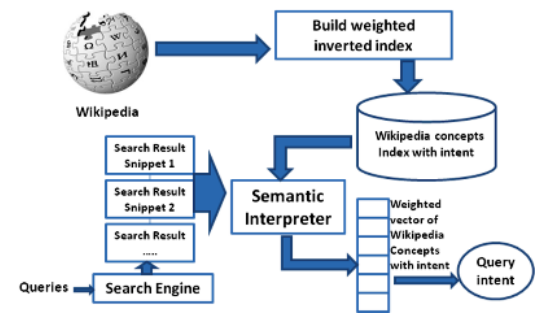
\includegraphics[scale=0.45]{img/wiki-intent-prediction}
\caption{The process of intent prediction}
\label{fig:wiki}
\end{figure}

The paper highlights few important patterns and anti-patterns followed in the methodology.\\

\textbf{Patterns:}
\begin{itemize}
\item In predicting future unseen data, two conditions should be satisfied: discriminative feature 
representation and sufficient training samples.
\item For query intents not covered by wikipedia, explicit semantic analysis (ESA) is used, which utilizes
Wikipedia for feature generation for the task of computing semantic relatedness. Empirical evaluation 
indicates that using ESA leads to substantial improvements in computing relatedness between words and text, 
and the correlation of computed relatedness of ESA with human judgments is much better than previous states
of the art.
\item \textit{TF-IDF} is used to quantify relation between words and concepts. An inverted index is constructed,
to speed up the semantic interpreter which maps each word into a list of Wikipedia concepts in which it appears.
\end{itemize}

\textbf{Anti-Patterns:}
\begin{itemize}
\item If the training data is too sparse, for query intent classification, discriminative feature representation
and sufficient training samples are hardly met together.
\item If the input samples only cover a subset of concepts in an intent domain, the learned classifier cannot
make good predictions for those queries that are not covered by the training samples.
\item If a user's input query is ambiguous according to the Wikipedia disambiguation pages, the method will not
make any intent prediction for this query.
\end{itemize}

The methodology proposed in this paper is very novel with their usage of wikipedia paving way for other techniques
like using search engines \cite{gibiec10}. This approach might have been a little ahead of time and would have 
yielded better results now and require much lesser manual effort since Wikipedia has improved significantly 
over the last 7 years.

\subsection{Machine Learning Techniques}
\label{sec:MLTechs}
\textit{Cleland-Huang et al.} proposed a machine learning approach to trace regulatory codes to product
specifications \cite{clelandHuang10}. This was published in International Conference on Software Engineering
and an extension to their earlier work \cite{clelandHuang05}.
Prior to this paper, methods for checking requirements compliance rely on standard software engineering practices of requirements traceability which is the ability to track a requirement from its origins back to its rationale and downstream to various work products that implement that requirement in software. Manual tracing can be prohibitively time-consuming; however automated trace retrieval methods are not very effective due to the vocabulary mismatches that often occur between regulatory codes and product level requirements. Studies show that organizations struggle to implement successful and cost-effective traceability, primarily because creating, maintaining, and using traces is a time-consuming, costly, arduous, and error prone activity. Moreover efficient information retrieval and data mining techniques have not been explored based on the literature which leaves an avenue open.

Two methods were proposed in the paper.

\textbf{Machine Learning Approach:} A training set of regulatory codes, product level requirements, and
their associated traces is constructed. A probabilistic weight is assigned to each term found in the
requirements with respect to each of the regulatory codes. This weight reflects the degree to which
a term represents a specific regulatory code. Each regulatory code is then categorized into a requirement 
based on this probabilistic weight score.

\textbf{Web Mining Approach:} It is based on the idea that when a training set is not available, a 
relevant set of indicator terms can be learned from domain specific documents mined from the Internet.
The benefit of the web-mining approach is that it bypasses the time-consuming step of manually constructing
a training set. The approach involves three steps. First a set of relevant domain specific documents are
identified. Second, the documents are analyzed to extract a set of domain specific terms. Finally these
terms are composed into a new query which is used to execute the trace.

This paper also illustrates a few patterns and anti-patterns.
\textbf{Patterns:}
\begin{itemize}
\item Automated methods have generally been quite effective, returning a candidate set of traces that 
contain 85- 90\% of the targeted links at precision rates of 10-50\%.
\item Although precision was low, basic automated methods excluded a large number of unlikely links.
\item For the machine learning approach, from a series of initial experiments selecting the top 10 
terms for each of the requirement types returned optimal classification results in comparison to other
selection methods.
\item Concept Generality threshold for a term is optimal at 0.3 and the maximum Domain Specificity for
a term is set to 5.
\end{itemize}

\textbf{Anti-Patterns:}
\begin{itemize}
\item Automated methods have limited success for tracing regulatory codes due to the significant disparity
in terminology that can exist between the codes and product level requirements.
\item Basic Automated methods yielded low precision values(Range of 0.02)
\item Additional error is introduced when human analysts are asked to evaluate a long list of candidate 
links generated by the automated methods.
\end{itemize}

This paper is one of the most highly cited papers in the domain with over 100 citations since 2010. The methods
in this paper are very novel and was explored in detail by other authors \cite{gibiec10}. This work addressed the
long existing low precision problem in the domain of requirements traceability. The authors could have used 
techniques more sophisticated to Pearson's Correlation to compare the techniques, for eg. non-parametric tests.

\begin{figure*}[htbp]
\begin{minipage}{\linewidth}
\centering
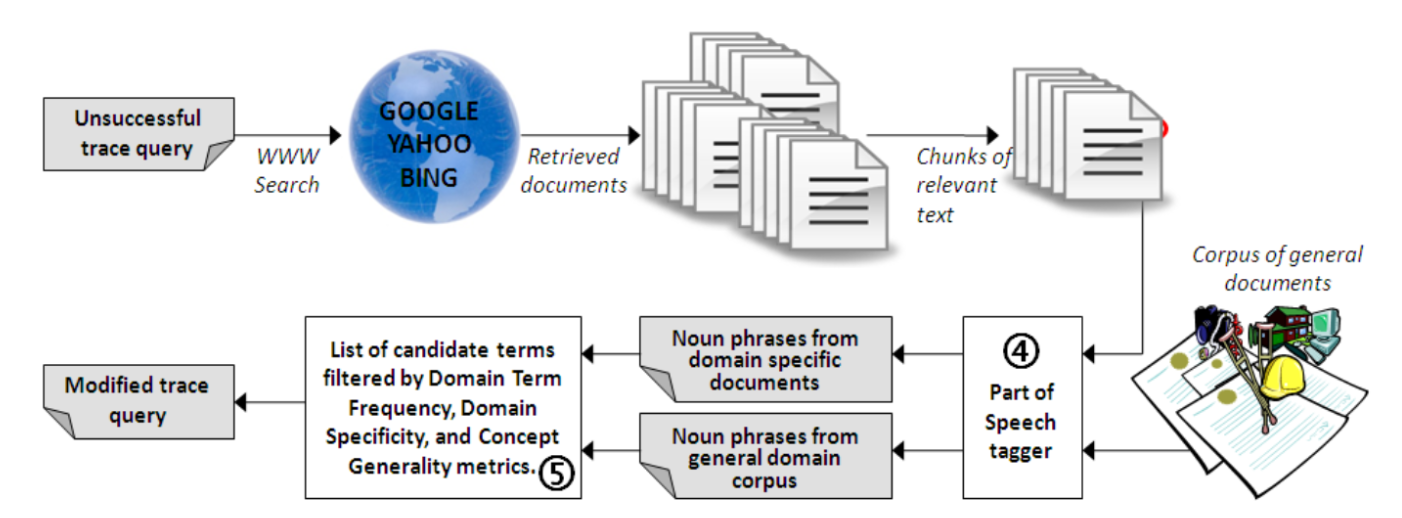
\includegraphics[scale=0.75]{img/query-modification}
\caption{Query Modification Technique.}
\label{fig:queryMod}
\end{minipage}
\end{figure*}

\subsection{Search Engines Augmentation}
\label{sec:SEAugment}
\textit{Gibiec et al.} explored mining replacement queries for ``hard to retrieve" traces in their
2010 publication in International Conference on Automated Software Engineering \cite{gibiec10}. They 
proposed using web search engines to obtain ideal replacement queries.

Automated Trace retrieval methods significantly reduce cost and effort involved in requirement traces. 
But many a times, it is not possible to find relevant links for a query. In such cases a human needs to
intervene to manually search for relevant links by modifying the query and/or rejecting links that are not
helpful. In many non-trivial projects the number of search links are very large(in order of thousands). In
such cases, it is hard to manually select or reject links. Techniques like Latent Semantic Indexing,
Vector space models and probabilistic approaches show that although the traceability effort in projects
are reduced, the traces generated are not very precise and additionally required an analyst to evaluated
the results to obtain the right set of links.

Based on the initial motivation and relevant work, the authors observed that low precision was caused due to a few stubborn results which reduced the overall quality of the generated results. Based on the paper,
stubborn traces occur when language in the document neither matches the language of the source document
nor matches the project level synonyms defined in a thesaurus. The paper addresses automating the web
mining process using various search engines and implementing and validating a technique for identifying
appropriate sections of text from retrieved documents.

Figure \ref{fig:queryMod} describes the query modification technique proposed by the authors. The text
from a stubborn trace query is used to seed a series of web searches using one or more standard search
engines. The retrieved documents are then filtered to remove documents which are difficult to parse
because they are primarily graphical in nature or which contain primarily advertisements. Each of the
retrieved documents is partitioned into smaller sections through splitting the document into overlapping
chunks of length \textit{chunkLength}. From the chunks, terms are then extracted using a \textit{Parts of
Speech} tagger. The terms are then used to compute the following metrics\\
\textbf{Domain term frequency:} It is the normalized term frequency information for each term across
multiple documents.\\
\textbf{Domain specificity:} It measures the extent to which a term or term phrase is specific to the domain document, as opposed to occurring frequently across a broad spectrum of topics.\\
\textbf{Concept generality:} This measure computes the fraction of domain specific documents in which a
specific term occurs. Concept generality differentiates between terms that occur in multiple domain
specific documents versus those that occur in only a few. \\
Once these metrics are computed, they are used to filter out non-useful terms. The remaining terms are
then ranked in descending order of term frequency.

The approach proposed in this paper is a fusion of \cite{clelandHuang10} and \cite{huWiki09}. The paper
does not justify why the authors needed to use three search engines as it does not make a significant
difference on the choice of the search engine. Along with precision and recall, measures of false alarm rate and F1 score would have given a better insight on the results.

\subsection{Enhancing Candidate Links}
\label{sec:enhanceCandidates}
\textit{Niu et. al} proposed using clustering for enhancing candidate links \cite{niu12}. Their work was 
published in IEEE International Conference on Requirements Engineering 2012.

Traceability has since been shown to be critical for a wide variety of software engineering activities,
including verification and validation (V\&V), risk assessment, and change impact analysis. However,
practitioners often fail to implement consistent and effective traceability processes if the traces are
maintained manually. Currently, IR-based tracing tools favor recall over precision. This is mainly because
commission errors (false positives) are easier to deal with than omission errors (false negatives)
\cite{hayes06}. However, retrieving an excessive number of links can seriously affect the practicality of
such tools. Due to the inherent trade-off between recall and precision, information retrieval methods
cannot achieve a high coverage without also retrieving a great number of false positives, causing a
significant drop in result accuracy.

Figure \ref{fig:clustering} illustrates the process of enhancing candidate link generation over
conventional IR-based tracing process. The authors suggest as follows:
\begin{itemize}
\item Clustering is performed after initial search is completed.
This makes the clustering dynamic rather than
static, i.e., they do not assume that if two artifacts $L_1$ and
$L_2$ are both correct or incorrect links for requirement
$R_A$, they must both be correct or incorrect links for
$R_B$. The link clusters produced in the approach are
query-dependent, and therefore have the potential to be 
closely tailored to the characteristics of the specific
requirement being traced.
\item Upon the identification of a cluster that divides correct
and incorrect links into separate groups, it is crucial
to research automated ways to differentiate between
high- and low-quality clusters. They propose several
heuristics and test their performance empirically.
\item Filtering in their approach does not rely solely on a link's
similarity to the query, but takes into account the cluster
the link belongs to as well \textit{i.e} a link's
neighbors also define its relevance. Filtering is thus
performed on a cluster basis, which is fundamentally
different from the baseline pruning strategy of acting
on individual links according to their similarity scores
or rankings.
\end{itemize}

\begin{figure}
\centering
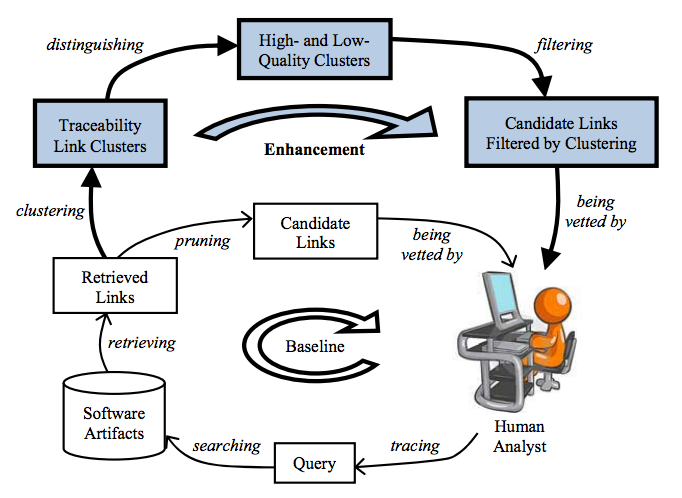
\includegraphics[scale=0.7]{img/clustering}
\caption{A clustering-based approach to enhancing candidate link
generation for requirements tracing. The bottom “baseline” cycle illustrates
a conventional IR-based tracing process. The three shaded boxes on the top
introduce the ``enhancement" steps derived from the cluster hypothesis.}
\label{fig:clustering}
\end{figure}

This paper also illustrates a few patterns and anti-patterns.\\
\textbf{Patterns:}

\begin{itemize}
\item To improve system performance clustering is first performed and then the query is matched to the
cluster centroids
\item Organizing and displaying the retrieved artifacts in topic-coherent clusters can facilitate the
comprehension and evaluation of the search results.
\item Pruning false positives to filter the result list can present the human analyst only a subset of
retrieved links.
\item Clustering is performed only after initial search. This makes clustering dynamic rather than static.
\item Heuristics can be used automatically differentiate between high quality and low quality clusters.
\item Filtering a link considers the similarity to the query as well as the cluster the link belongs to.
\end{itemize}

\textbf{Anti-Patterns:}

\begin{itemize}
\item As the number of documents increases, matching the query to all documents can degrade the system
performance.
\item The searchable artifacts in tracing consist of individual requirements, classes and test cases. Such
a collection tends to be significantly smaller than the document collection targeted in a typical Web
search or online library search. Therefore, the need of reducing the search space via document clustering
is less pressing in requirements tracing.
\item Ideally every requirement is concise, primitive, and unambiguous, the reality is that requirements 
can often be relatively long and may also contain superfluous information.
\end{itemize}

The approach taken by the authors were further extended by them \cite{niu13} and also
\textit{Cleland-Huang et al.} \cite{clelandHuang14}. The research questions in the paper could have been
addressed explicitly. It would have made identifying the solutions of the research questions easier. Also,
the authors did not mention the intuition behind selecting the proposed clustering methods. The approach
of using clustering based methods yields better precision scores along with recall and is very novel. The
datasets used for their experiments are described in Sections \ref{sec:ds:iTrust} and \ref{sec:ds:cm1}.


\subsection{Query Reformulation}
\label{sec:queryReformulate}
\textit{Haiduc et al..} developed a tool ``Refoqus" to predict the quality of the query and reformulate it
for source code search \cite{haiducRefoqus13}. This work of theirs was published in International
Conference of Software Engineering 2013.

\begin{figure}
\centering
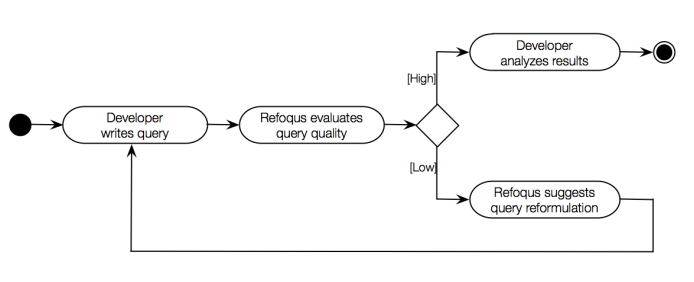
\includegraphics[scale=0.7]{img/refoqus}
\caption{Workflow of Refoqus}
\label{fig:refoqus}
\end{figure}

The problem common to all Text Retrieval based approaches is that the text query used and its relationship
to the text contained in the software artifacts greatly influences the search results. Writing good
queries is not an easy task as it requires intimate knowledge of the source code vocabulary and its use,
which is difficult to get even in small projects, let alone in large projects with millions of lines of code.
A poor query not only fails to return relevant results, but it also leads to wasted time and effort
on behalf of the developers, who need to investigate the irrelevant search results before realizing that
the query was a poor choice. The challenge is to provide immediate feedback about quality of the query.

Query reformulation is often very difficult for developers, given that they do not know how to write an
optimal query. Researchers in the SE field have addressed this problem by proposing the use of two types
of query reformulation approaches. The first is based on user relevance feedback, which is an interactive
approach that relies on the developer to analyze the list of results and mark the top documents as
relevant or not relevant \cite{deLucia06}. The documents marked by the user are then used to reformulate
the query. One disadvantage of this technique is that it requires significant developer effort for
analyzing and marking documents that are not directly relevant for the task at hand. A second class of
approaches is based on automatically adding terms to the query, which are similar to the terms found in
the query (e.g., synonyms) \cite{gibiec10}.

Refoqus stands for REFormulation of QUerieS and uses a combination of techniques from the fields of
natural language document retrieval and machine learning. The proposed approach uses 21 measures
reflecting textual characteristics of the query and of the entire source code to determine if the written
query is of high or low quality. The quality prediction is based on training the system using existing
examples of good and poor queries. Refoqus also uses additional measures, which convey information about
the results returned by the query: Subquery Overlap, Robustness Score, First Rank Change, Clustering
Tendency, Spatial Autocorrelation, Weighted Information Gain, and Normalized Query Commitment. They are
defined in the field of natural language document retrieval and their use in SE context is a first. Using
these additional sources of information leads to better quality prediction in Refoqus.

Refoqus is meant to be used by developers during their daily tasks, whenever searching is needed.The work
flow of Refoqus is illustrated in Figure \ref{fig:refoqus}. Refoqus works like any other TR-based tool for
source code search, i.e., the developer writes and runs a text query and Refoqus returns a list of ranked
methods relevant to the query. While retrieving the relevant results, Refoqus also analyzes the quality of
the submitted query and classifies it as high or low quality. The developer can use this feedback as a
guideline for determining if the results returned by the query are worth investigating or not. In the case
when Refoqus indicates the query is of high quality, the developer is likely to find the relevant code
among the top results and the search can end successfully. In case the quality of the query is low, the
developer is most likely better off reformulating the query than analyzing the search results. In such
cases, Refoqus automatically suggests a reformulation of the query.

The tool refoqus is very well documented and also has a youtube
video\footnote{\url{http://www.youtube.com/watch?v=UQlWGiauyk4}} describing its use. The paper does provide a
base tool to compare refoqus with nor does it mention if a similar tool has been previously been 
developed by the research community. The authors describe the performance of the tool using accuracy. 
Using precision or recall instead would have given a better insight on the performance of the tool.



\subsection{Intelligent Trace Retrieval}
\label{sec:intelligentTraces}
\textit{Cleland-Huang et al.} gave their insights on what approaches could be taken towards more 
intelligent trace retrieval algorithms\cite{clelandHuang14}. This work was published in the 
International Workshop on Realizing Artificial Intelligence Synergies in Software Engineering.

Vast majority of relevant work in the past decade has been focused at the lowest level of the
Traceability Intelligence Quotient (tIQ) and posit that achieving high quality automated traceability
will require re-focusing research efforts on the development of more intelligent algorithms capable
of reasoning about concepts, their relationships and constraints, and the contexts in which they occur.
Traditional approaches to traceability, including those integrated into most commercial tools,
assume that users will create and maintain trace links manually. Unfortunately, the authors believe
the tracing task are arduous and error-prone and therefore in practice even the most basic trace links
are found to be inaccurate, incomplete, and ambiguous.

Information retrieval techniques are used to compute similarity scores (or link probabilities) between
pairs of source and target artifacts, such as between requirements and code, or between regulations and
requirements, and then to present high-scoring pairs as candidate links to users. The authors propose a
classification scheme which identifies various degrees of intelligence exhibited by text-centric trace 
creation algorithms and posit that continued efforts to achieve high degrees of automation will require
focusing our efforts on developing more intelligent tracing solutions. They choose to focus purely on 
text-based techniques because these are a core component of almost every automated, or semi-automated
tracing algorithm.

They define a parameter called ``Traceablity Intelligence Quotient"(tIQ) and summarize on an ordinal
scale that includes the abilities like
\begin{itemize}
\item \textbf{Term Matching:} The notion is that trace links can be constructed when terms in the 
source artifact match those in the target artifact. The most popular approach is based on the Vector
Space Model (VSM). Techniques such as Latent Semantic Indexing (LSI) or Latent Dirichlet Allocation
(LDA) overcome the strict term-to-term matching of the VSM through using processes such as Singular
Value Decomposition to discover simple associations between terms by extracting and leveraging the
contextual usage of each word.
\item \textbf{Basic Untyped Associations:} Techniques that fall into this category are characterized
by the fact that they do not understand the semantics behind the association. An example in the 
traceability domain is based on learning query transformation rules from an initial set of approved 
trace links. Another example uses either structural or term-based clustering to leverage the general
idea that groups of similar items tend to be linked to other groups of similar items.
\item \textbf{Semantic Associations:} Semantic Associations utilizes a Knowledge Base to create and
utilize semantically aware associations in the trace creation process. Such knowledge bases are composed
of a set of data that includes basic terms that define the vocabulary of the domain, and a set of 
sentences that describe the relationships between those terms. The data is often represented in the 
form of an ontology in which knowledge is constructed using logical operators such as AND and OR,
as well as implication and negation operators to build complex ideas from more primitive concepts.
\item \textbf{Expert Systems:} An expert system emulates the decision-making process of a human expert.
Expert traceability systems are therefore designed to closely mimic the way human analysts reason about
trace links and perform tracing tasks. Such systems rely on a knowledge base (ontology) which understands
the vocabulary, facts, and assumptions of the domain and represents them in a format that is accessible
and processable. There is currently little work in this area.
\item \textbf{Knowledge Synthesis:} These represents class of algorithms which have the ability to 
synthesize information in order to address the question of when each different technique should be used,
and how various techniques can be combined. True synthesis of knowledge will only be effective when
intelligent traceability solutions from higher levels of our tIQ classification are thrown into the mix.
\end{itemize}

For their experiments, they searched DBLP\footnote{http://dblp.uni-trier.de/db/} for all listed papers 
from 2004-2013 including the term "Traceability" in either the title, abstract, or list of keywords. 
DBLP includes the top ranking conferences and journals in which traceability related work typically
occurs, such as the International Conference on Software Engineering (ICSE), the Requirements Engineering
Conference (RE), the International Conference on Software Maintenance (ICSM), the Automated Software 
Engineering Conference (ASE), Foundations of Software Engineering (FSE) or the European Software 
Engineering Conference (ESEC), IEEE Software, ACM Transactions on Software Engineering Methodology 
(TOSEM), and IEEE Transactions on Software En- gineering (TSE). This search returned 696 results. Any 
paper related to execution traces or traceability of farm products (or similar) rather than trace 
retrieval were removed, resulting in a total of 395 papers. They then further narrowed the selection by 
retaining only those papers which talked about automated trace creation or maintenance. Furthermore, if 
the underlying trace retrieval algorithm was not clearly explained, typically because the emphasis was 
on traceability processes or the application of traceability to a specific task, they also eliminated the
paper. They were left with a set of 107 papers. Each paper was then classified according to the highest
possible level of the tIQ.

This work provides a comprehensive study on the state of the art traceability methods and their drawbacks
as of 2014. Although the authors mention that they have summarized only approaches using only text mining,
they have given a high level insight on other forms of trace retrieval methods. The authors could have 
published the resource to the data collected for their study as it would have augmented the research 
community. In the future work section of the paper, the authors could have provided an intution on
how to approach the active problems.

\section{Data Sets}
\label{sec:datasets}
\subsection{Ice Breaker Systems}
\label{sec:ds:IBS}
The proposed methods in Section \ref{sec:dynamicReq} focused on the retrieval of links between
requirements and UML class diagrams in order to simulate the type of traceability performed during
an impact analysis query. The Ice Breaker System (IBS) was initially described in 
\cite{robertson99} and enhanced with requirements mined from documents obtained from the public
work departments of Charlotte, Colorado; Greeley, Colorado; and the Region of Peel, Ontario. IBS
manages de-icing services to prevent ice formation on roads, receiving inputs from a series
of weather stations and road sensors within a specified district, and using this information
to forecast freezing conditions and schedule dispersion of salt and other de-icing materials.
It maintains maps of the district, plans de-icing, manages the inventory of de-icing
materials; maintains, dispatches, and tracks trucks in real time; and issues and tracks work 
orders. The Ice Breaker system consists of 180 functional requirements, 72 classes, and 18 packages.

\subsection{iTrust}
\label{sec:ds:iTrust}
iTrust\footnote{\url{http://agile.csc.ncsu.edu/iTrust}} is a medical application developed by the students
from North Carolina State University (USA). iTrust is a medical application that provides patients with a
means to keep up with their medical history and records as well as communicate with their doctors, 
including selecting which doctors to be their primary caregiver, seeing and sharing satisfaction results,
and other tasks. iTrust is also an interface for medical staff from various locations. iTrust allows the
staff to keep track of their patients through messaging capabilities, scheduling of office visits, 
diagnoses, prescribing medication, ordering and viewing lab results, among other functions.

\subsection{CM1}
\label{sec:ds:cm1}
CM1\footnote{\url{http://promise.site.uottawa.ca/SERepository/datasets/cm1.desc}} contains a complete set
of requirements (high-level) and design (low-level) documents for a NASA scientific instrument. The
dataset contains 235 high level and 220 low-level requirements. The trace for the dataset was manually
verified. The "theoretical true trace" (answerset) built for this dataset consisted of 361 correct links.
Each of the high and low-level files contain the text of one requirement element.

\section{Future Work}
\label{sec:future}
Although the current automatic methods for trace retrieval have high recall, most proposed methods suffer low precision values. Thus, very few valid traces will be returned to the user. This is a challenge which would be of highest priority. In 2011, \textit{Glorot et al.} published in AISTATS on using Deep Sparse Rectifier Neural Networks for text mining\cite{glorot11}. This method yielded good precision values for large corpora and could be experimented on requirement traces. Recently, \textit{Nguyen et al.} reported promising results in mining code APIs using statistical models\cite{nguyen14}. This method could also be experimented on mining traces.

Requirement trace mining is bound to be a computationally intensive process and researchers could focus on improving the runtimes for the state of the art algorithms. Parallel computing could be a great starting point. Systems such as HPC-LSF\footnote{\url{https://en.wikipedia.org/wiki/Platform_LSF}} and CUDA\footnote{\url{https://en.wikipedia.org/wiki/CUDA}} would be ideal for such compute intensive approaches.

% \section{Conclusions}
% This paragraph will end the body of this sample document.
% Remember that you might still have Acknowledgments or
% Appendices; brief samples of these
% follow.  There is still the Bibliography to deal with; and
% we will make a disclaimer about that here: with the exception
% of the reference to the \LaTeX\ book, the citations in
% this paper are to articles which have nothing to
% do with the present subject and are used as
% examples only.
%\end{document}  % This is where a 'short' article might terminate

%ACKNOWLEDGMENTS are optional
\section{Acknowledgments}
This report is part of CSC-791 Automated Software Engineering. The author would like to express my gratitude towards the instructor Dr Tim Menzies and the Teaching Assistant Rahul Krishna for the their support in pursuing this project. All figures used in this paper are part of the source paper which was summarized and do not belong to the author or the teaching staff of the course.

%
% The following two commands are all you need in the
% initial runs of your .tex file to
% produce the bibliography for the citations in your paper.
\bibliographystyle{abbrv}
\bibliography{refs}  % sigproc.bib is the name of the Bibliography in this case
\end{document}
